The usage area is how various actors interact with the system, and through that controls, documents, and observes the problem area. Actors can be any exterior entity which is connected to the usage of the system, like people, but also includes external systems. These actors have various patterns of use available to be them, which lets them perform actions with the system.

\textbf{Actors \& Patterns of Use}

For this system there is only two kind of actors: The ‘user’, and what has been named call the ‘updater’.

The user is the general media interested person who uses the system to find media which he might be interested in, which is his purpose in the context of the system. He has a medialist, where he rates and indicates media, which he has consumed. He also have a friendlies where he makes connections with other people he know, or through their common interest. The unique characteristic of a user is their medialist and preferences, which can alter the recommendations process, generating different results.

The updater is an external system. Its purpose is to update the media which the system has available to it, with information coming from various sources. This is done to keep the system updated for newly released media, and made available for the users to add to their medialists. The characteristic of an updater is the media type which it keeps track of, and the sources which it extracts these data from.

The patterns of use is the various actions which is the actors can perform in the usage area. The patterns of use for this is: See medialist, see friendlist, indicate/rate media, remove media, add friend, remove friend, update media collection. These have been made into a table, with actors, indicating which pattern of use belongs to which actor. See Table \ref{UseTable}.

Among these you could also include a pattern of use called ‘Generate recommendations’. This depends on how this use is actually activated, as it may not be the most sensible choice to have this available to all users. The more sensible choice would be to activate it in certain intervals, to avoid a user abusing the action, possible slowing or crashing the system from overwork. In this it will be excluded.

\begin{table}[htb]
\centering
\begin{tabular}{|l|c|c|} \hline
	  & \textbf{User} & \textbf{Updater} \\ \hline
	\textbf{See Medialist} & X &  \\ \hline
	\textbf{See Friendlies} & X &  \\ \hline
	\textbf{Indicate/Rate Media} & X &  \\ \hline
	\textbf{Remove Media} & X &  \\ \hline
	\textbf{Add Friend} & X &  \\ \hline
	\textbf{Remove Friend} & X &  \\ \hline
	\textbf{Update Media Collection} &  & X \\ \hline
\end{tabular}
\caption{Pattern of Use table}
\label{UseTable}
\end{table}

The following two figures shows patterns of use, indicate/rate media, and update media collections. These two were singled out for being the more unique patterns of use among those available, and the more crucial among them. See the first Figure \ref{IndicateMedia} for the indicate/rate media pattern of use, and Figure \ref{UpdateCollection} for the update media collection pattern of use.

\begin{figure}[htb]
\centering
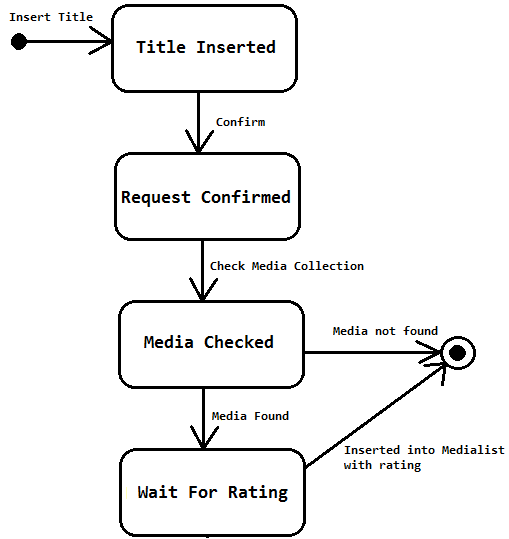
\includegraphics[width=0.5\textwidth]{Images/IndicateMedia.png}
\caption{Diagram of the Indicate/Rate media pattern of use}
\label{IndicateMedia}
\end{figure}

The indicate/rate media pattern of use is initiated by the user, when the user in questions wants to add a piece of media, together with a rating, to their medialist. The user inserts the title of a media, or some other defining characteristic, which then have to be confirmed before the pattern of use begins to check whether or not the piece of media exists in the systems collections. If the media was not in the collection, the pattern of use will stop. If they media was, it will wait for the user to indicate his rating for the media, and will then finish the pattern of use by saving it in the users medialist. Involved objects include the media interested person, and the media objects.

\begin{figure}[htb]
\centering
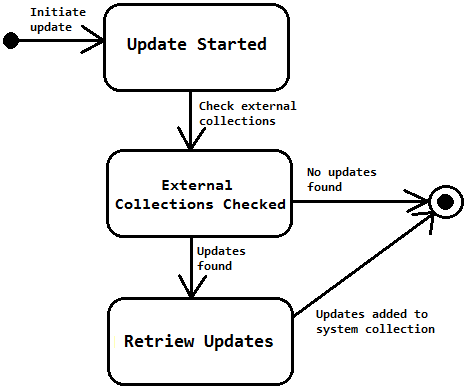
\includegraphics[width=0.5\textwidth]{Images/UpdateCollection.png}
\caption{Diagram of the Update Media Collection pattern of use}
\label{UpdateCollection}
\end{figure}

The update media collection is either initiated in a certain interval, or when new media content is detected available for the system. This case shows the former possibility. This pattern of use starts by checking external collections upon being initiated, and will either end if no new media content was detected, or will begin retrieving said media content. After retrieving the media updated from the external collections, the pattern of use will end by adding the media updates to the systems collections. Involved objects are several media objects.

\textbf{Functions}

Functions is the methods which is stands for most of the systems processing of data, and makes it possible for actors to communicate with the model of the system, through this function layer. Functions can include any of the patterns of use which has already been described, but there can also be additional functions, depending on the context of the system. For this system, there is a function called ‘Generate Recommendations’, which was excluded from the patterns of use on this case, but is still very crucial for the system. 

Functions are divided into four types: Update, read, calculate, and signal.
\begin{itemize}
	\item Update Functions
	\begin{itemize}
		\item Indicate/Rate media, remove media, add friend, remove friend, update media collection.
	\end{itemize}
	\item Read Functions
	\begin{itemize}
		\item See media, see friends, search for
	\end{itemize}
	\item Signal \& Calculate Functions
	\begin{itemize}
		\item Generate recommendations
	\end{itemize}
\end{itemize}

In this context, the generate recommendations function can easily go as both a signal and calculate function, as it has properties of both kinds. It processes data from the model, and generates recommendations based on this data, and then makes it viewable for the user, through the ‘See media’ function. The function itself is activated by a signal, like the user logging into their account, or a planned interval, generating the recommendations outside of the users consent.

These functions is then put into a table, indicating their function type, and determine the complexity of every function. See Table \ref{FuncTable}.

\begin{table}[htb]
\centering
\begin{tabular}{|l|c|c|} \hline
	 \textbf{Function} & \textbf{Complexity} & \textbf{Type} \\ \hline
	Indicate/Rate Media & Medium & Update \\ \hline
	Remove Media & Medium & Update \\ \hline
	Add Friend & Simple & Update \\ \hline
	Remove Friend & Simple & Update \\ \hline
	Update Media Collection & Complex & Update \\ \hline
	See Media & Simple & Read \\ \hline
	See friends & Simple & Read \\ \hline
	Search For & Medium & Read \\ \hline
	Generate Recommendations & Very Complex & Signal/Calculation \\ \hline
\end{tabular}
\caption{Functions with their complexity and type}
\label{FuncTable}
\end{table}